\section{はじめに}

書いたプログラムが思った通りの挙動をしない時、プログラマはデバッグをする必要がある。

単純なデバッグはプログラムを実行した際の出力から推測したりソースコードを眺めることで行われるが、そのようなデバッグは「ソースコードのどの部分が間違っているか」を示すものが無く、多くの時間や労力を要することがある。特にプログラミングにまだ慣れていない初学者にとっては、デバッグの経験や言語に対する理解が乏しい為、より困難な作業になると考えられる。

そこで色々な言語にデバッガが用意されているが、デバッガを利用するには、デバッガのコマンドの文字列や意味を覚えたり、ブレイクポイントを設定する箇所を考えたりといった、初学者にとってやはり困難な操作が必要になる。また、一般的なデバッガで表示されるのは「ソースコード中の実行中の行」であり、どこで今の関数を呼び出されたのか、この後どんな計算があるのかなどといったプログラム全体の流れが分かりにくい。

\begin{figure}
  \begin{center}
    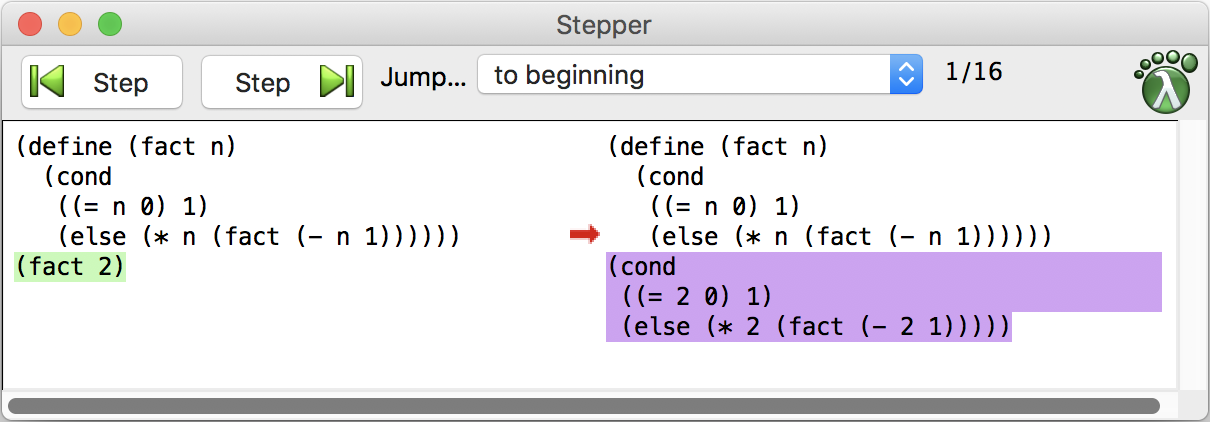
\includegraphics[width=13cm]{racket1.png}
  \end{center}
  \caption{DrRacket のステッパ}
  \label{figure:racket1}
\end{figure}

\begin{figure}
  \begin{center}
    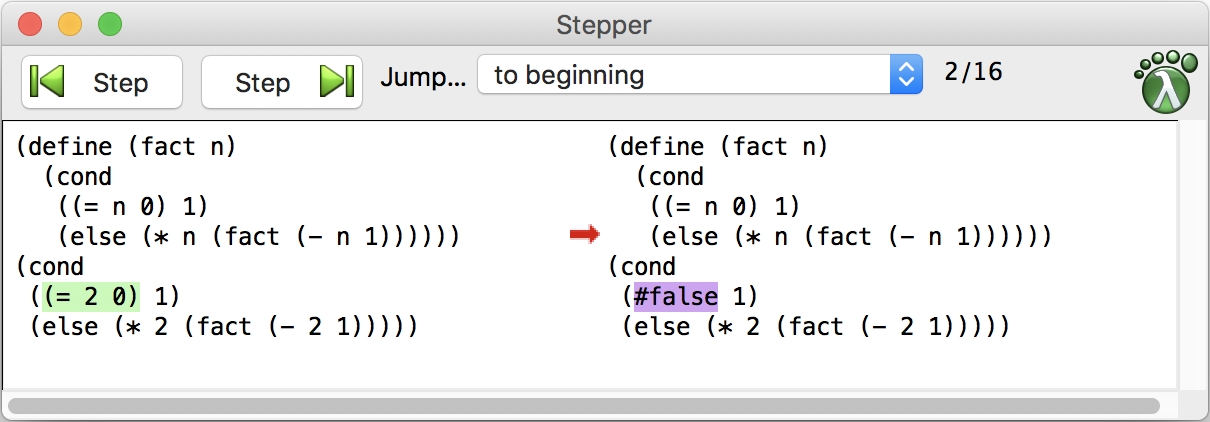
\includegraphics[width=13cm]{racket2.png}
  \end{center}
  \caption{DrRacket のステッパを進めた様子}
  \label{figure:racket2}
\end{figure}

我々は、プログラミング初心者がデバッグをするのに最適な方法は、ステッパを使うことだと考える。ステッパは Racket 言語の統合開発環境 DrRacket において提供されているツール\cite{clements01}である。ユーザがエディタにプログラムを書いてステッパ起動ボタンを押すと、図\ref{figure:racket1}のようなウインドウが表示される。図\ref{figure:racket1}は、再帰関数を用いて2の階乗を計算するプログラムを入力してステッパを起動したときの様子である。ウインドウには左右にそれぞれプログラムが表示されている。左はユーザが入力したプログラムと同じものであり、このプログラムで最初に簡約される式 \texttt{(fact 2)} が緑色にハイライトされている。右側のプログラムでは、ハイライトされた部分以外は左側と同じプログラムが表示されており、左側では緑色だった式 \texttt{(fact 2)} がその簡約結果に置き換えられ、紫色でハイライトされている。

Step ボタンのうち右の実行を進めるボタンを押すと図\ref{figure:racket2}のような表示に切り替わる。最初(図\ref{figure:racket1})は右側にあったプログラムと同じプログラムが左に表示され、次に簡約される部分式 \texttt{(= 2 0)} が緑色にハイライトされており、右側には同様にその部分が簡約されて紫色になったプログラムが表示されている。当初 \texttt{(fact 2)} だった式がその値である \texttt{2} になるステップまで、ボタンを押すと次々に簡約が行われてプログラムが変形していく様子を視覚的に見ることができる。

このように、プログラムを実行したときに、実行結果の値だけでなく、実行中にプログラムが代数的にどのように書き換えられていくかを見せるツールがステッパである。ステッパの操作は基本的に「前のステップへ」「次のステップへ」のボタンを押すのみであり、プログラミングや CUI での操作に慣れていない初心者でも使いやすい。

しかし、DrRacket のステッパが受け付けるのは Racket 言語のうちの一部の構文で構成された教育用の言語であり、例外処理などがサポートされていない。初心者にとって理解しにくい例外処理をステップ実行できるようにするため、著者らは関数型言語 OCaml の、例外処理を含む基礎的な構文に対応したステッパを実装し評価した\cite{FCA18}。簡約される式のハイライトなどの表示の仕方は、概ね DrRacket のステッパ\cite{clements01}と同様にした。

そのステッパを実際に OCaml の初学者に利用してもらった\cite{FCA18}ところ、ステッパが再帰関数などの理解に役立ったことが分かったが、「プログラムの実行が終わってからインタフェースの動作が始まるので、実行に時間がかかるプログラムを実行しようとすると最初のステップが長時間表示されず利用できない」という問題があった。

本研究では、1度のステッパプログラムの実行で1ステップを実行するように変更し、プログラム全体の実行時間にかかわらずステップ実行ができるステッパを構築する。それによって実行に時間のかかる例外処理を含むプログラムのステップ実行ができるほか、ステッパをクライアントサーバ方式で実装することが可能になる。
